\chapter{Technology: Architecture and Scalability}

\section{Defining a Scalable Tech Strategy}

A scalable technology strategy is foundational to any growing organization. A well-architected strategy ensures that the system can handle increased loads, adapt to changing business requirements, and maintain efficiency as the company evolves. This section explores key elements such as technology selection, evaluation, and future-proofing systems.

\subsection{Technology Selection and Evaluation}

Choosing the right technology stack is critical for long-term scalability and maintainability. The decision-making process should be systematic, taking into account technical and business factors.

\textbf{Key Factors in Technology Selection:}
\begin{itemize}
    \item \textbf{Performance:} Ensuring the selected technology meets required latency and throughput demands.
    \item \textbf{Scalability:} Assessing how well the technology scales horizontally and vertically.
    \item \textbf{Community and Support:} Evaluating the ecosystem, documentation, and vendor support.
    \item \textbf{Security:} Ensuring compliance with industry standards and security best practices \index{security}.
    \item \textbf{Total Cost of Ownership (TCO):} Considering licensing, operational, and maintenance costs.
\end{itemize}

A comparison table can help in technology evaluation:

\begin{table}[ht]
    \centering
    \begin{tabular}{|l|c|c|c|}
        \hline
        \textbf{Criteria} & \textbf{Technology A} & \textbf{Technology B} & \textbf{Technology C} \\
        \hline
        Performance       & High                  & Medium                & Low                   \\
        Scalability       & High                  & High                  & Medium                \\
        Community Support & Strong                & Moderate              & Weak                  \\
        Cost              & Low                   & High                  & Medium                \\
        \hline
    \end{tabular}
    \caption{Technology Selection Matrix}
    \label{tab:tech_selection}
\end{table}

\subsection{Future-Proofing Systems}

Future-proofing technology ensures longevity and adaptability. Some key principles include:

\begin{itemize}
    \item \textbf{Modular Architecture:} Designing systems with clear separation of concerns (e.g., microservices\index{microservices}).
    \item \textbf{Loose Coupling:} Ensuring components communicate via well-defined APIs to minimize dependencies.
    \item \textbf{Backward Compatibility:} Designing systems that support legacy data and integrations.
    \item \textbf{Observability:} Embedding monitoring and logging for proactive issue resolution.
\end{itemize}

\section{Engineering Best Practices}

\subsection{Code Quality and Standards}

Code quality is essential for maintainability and collaboration. Best practices include:

\begin{itemize}
    \item \textbf{Consistent Coding Style:} Using linters and formatters (e.g., Prettier, ESLint).
    \item \textbf{Code Reviews:} Implementing peer reviews to catch bugs early.
    \item \textbf{Documentation:} Maintaining inline and API documentation.
\end{itemize}

\begin{tipbox}
    \textbf{Do not reinvent the wheel:} Programming languages and frameworks have established best practices. Follow them to ensure maintainability and readability.\\
    \\
    \textbf{TypeScript examples:}
    \begin{itemize}
        \item \url{https://docs.aws.amazon.com/prescriptive-guidance/latest/best-practices-cdk-typescript-iac/typescript-best-practices.html}
        \item \url{https://google.github.io/styleguide/tsguide.html}
    \end{itemize}
\end{tipbox}

\subsection{Testing and Automation}

Automated testing improves reliability and efficiency.

\begin{itemize}
    \item \textbf{Unit Tests:} Validating individual components.
    \item \textbf{Integration Tests:} Ensuring components work together.
    \item \textbf{Continuous Integration (CI):} Automating test execution on every commit.
\end{itemize}

\subsection{Security by Design}

Security should be embedded from the start.

\begin{itemize}
    \item \textbf{Threat Modeling:} Identifying potential vulnerabilities.
    \item \textbf{Least Privilege Principle:} Granting only necessary access.
    \item \textbf{Regular Audits:} Conducting security reviews and penetration testing.
\end{itemize}

\section{Infrastructure and Operations}

\subsection{Cloud vs. On-Premise Considerations}

Choosing between cloud\index{cloud} and on-premise\index{on-premise} solutions involves several trade-offs:

\begin{itemize}
    \item \textbf{Scalability:} Cloud solutions offer elastic scaling, whereas on-premise requires capacity planning.
    \item \textbf{Cost:} Cloud follows an OPEX model, while on-premise is typically CAPEX.
    \item \textbf{Control:} On-premise offers greater control over security and compliance.
\end{itemize}

\begin{figure}[h]
    \centering
    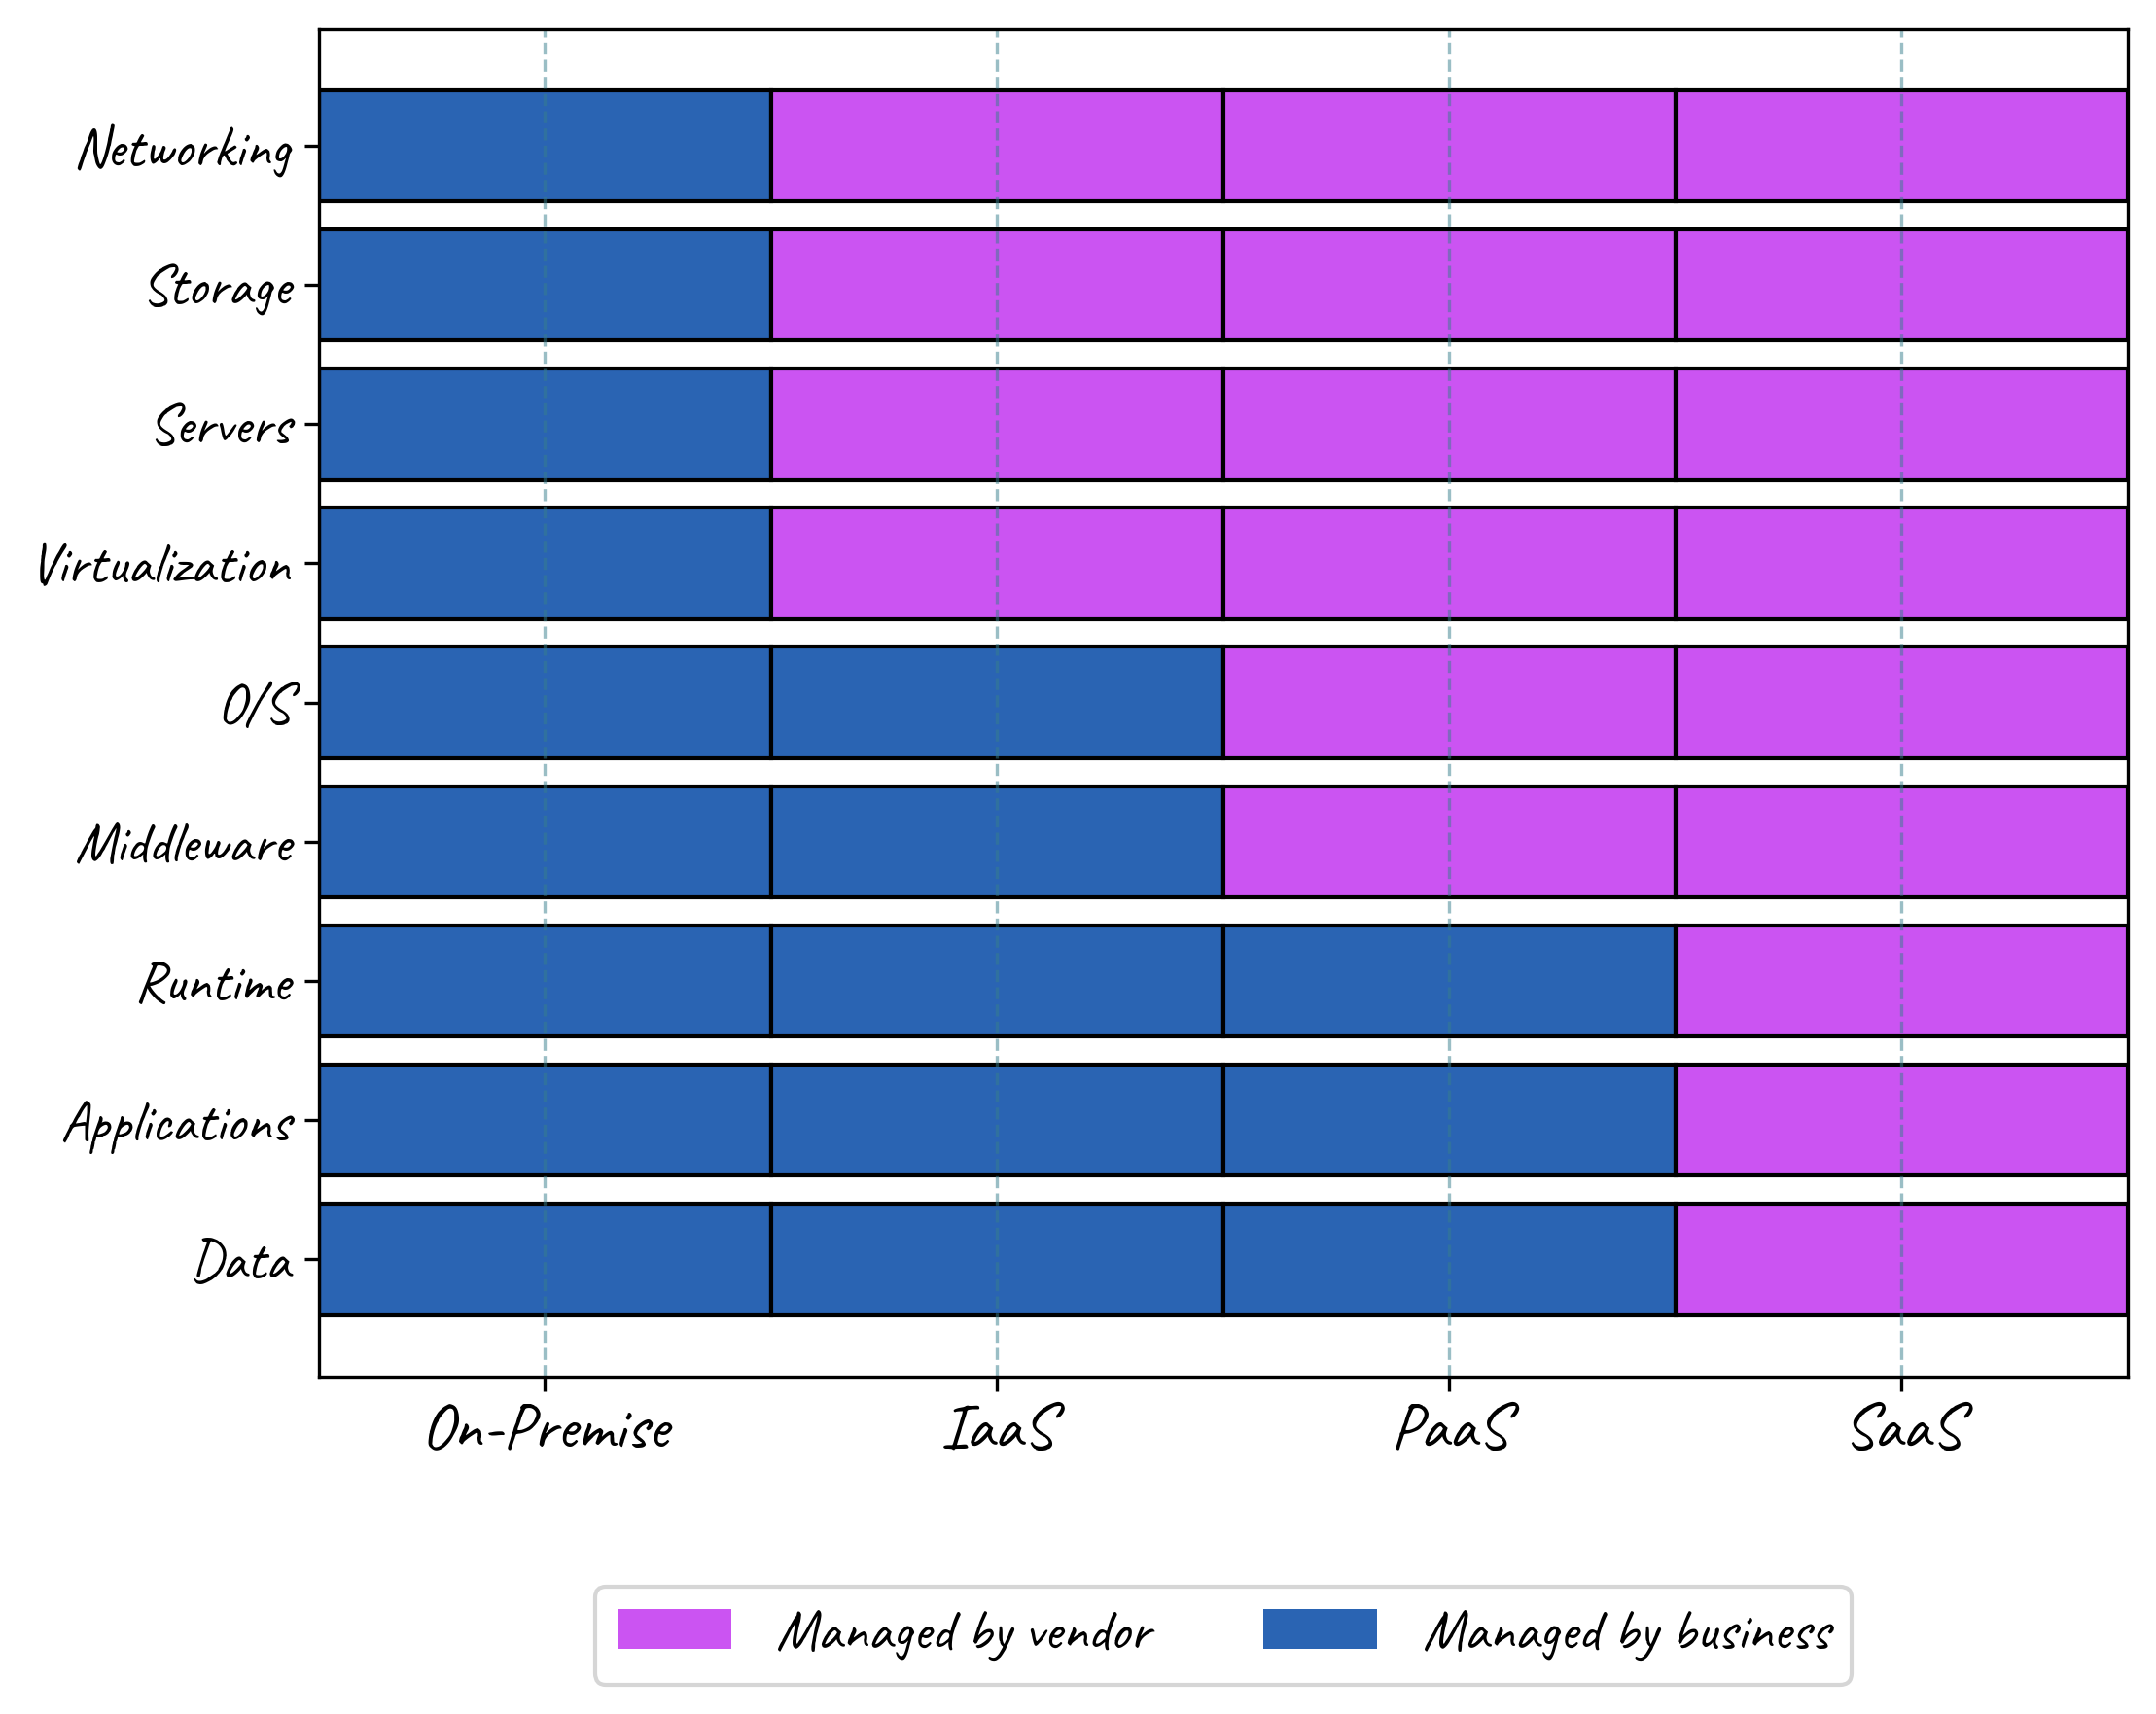
\includegraphics[width=0.8\textwidth]{infrastructure-models.png}
    \caption{Infrastructure models}
\end{figure}

\subsection{Observability and Monitoring}

Monitoring provides visibility into system health. Key components include:

\begin{itemize}
    \item \textbf{Metrics:} Measuring CPU, memory, latency.
    \item \textbf{Logging:} Centralized log aggregation (e.g., ELK stack).
    \item \textbf{Tracing:} Distributed tracing for debugging microservices.
\end{itemize}

\subsection{Incident Management and Reliability}

A structured approach to incident management is essential for maintaining system reliability and ensuring business continuity. As organisations increasingly depend on technology, a well-defined incident response process mitigates downtime, enhances resilience, and fosters continuous improvement.

\subsubsection{Incident Response Plan}

An effective incident response plan (IRP) provides predefined escalation paths, roles, and procedures that guide the organisation during a crisis. A comprehensive IRP typically includes the following key elements:

\begin{itemize}
    \item \textbf{Detection and Identification:} Implementing monitoring tools such as Prometheus, Datadog, or AWS CloudWatch to detect anomalies and trigger alerts.
    \item \textbf{Classification and Prioritisation:} Categorising incidents based on severity levels (e.g., P1, P2, P3) to ensure a proportionate response.
    \item \textbf{Escalation and Communication:} Defining communication protocols and using tools like PagerDuty or Slack to alert on-call engineers and stakeholders.
    \item \textbf{Resolution and Mitigation:} Applying predefined playbooks and automated remediation mechanisms to reduce mean time to resolution (MTTR).
    \item \textbf{Review and Documentation:} Capturing key incident details to inform future prevention strategies.
\end{itemize}

A well-structured IRP reduces confusion during crises and accelerates recovery, ensuring minimal impact on users and business operations.

\subsubsection{Postmortems and Continuous Learning}

Postmortems are essential for learning from past failures and improving reliability over time. A blameless postmortem culture fosters transparency and accountability while encouraging proactive risk mitigation. Key components of an effective postmortem include:

\begin{enumerate}
    \item \textbf{Incident Summary:} A clear description of the event, impact, and affected systems.
    \item \textbf{Root Cause Analysis (RCA):} Identification of underlying factors, often using methodologies such as the "Five Whys" or Fishbone Diagrams.
    \item \textbf{Timeline of Events:} A chronological breakdown of detection, response, and resolution actions.
    \item \textbf{Lessons Learned:} Insights gained from the incident, highlighting gaps in monitoring, automation, or communication.
    \item \textbf{Action Items:} Concrete steps to prevent recurrence, assigned to responsible teams with defined deadlines.
\end{enumerate}

Organisations such as Google and Netflix have adopted postmortem processes to enhance system reliability, demonstrating the effectiveness of continuous learning in technology operations \cite{allspaw2012postmortem}.

\subsubsection{Redundancy and High Availability}

Ensuring system reliability requires designing for failure through redundancy and high availability. This involves implementing fault-tolerant architectures that can withstand component failures without significant service degradation. Key strategies include:

\begin{table}[h]
    \centering
    \begin{tabular}{|l|p{10cm}|}
        \hline
        \textbf{Strategy}       & \textbf{Description}                                                                                      \\
        \hline
        Load Balancing          & Distributing traffic across multiple servers using tools like AWS ELB, Nginx, or HAProxy.                 \\
        \hline
        Database Replication    & Using primary-replica setups or multi-region replication in databases like PostgreSQL, MySQL, or MongoDB. \\
        \hline
        Multi-Cloud Deployments & Running services across multiple cloud providers (e.g., AWS and GCP) to mitigate cloud outages.           \\
        \hline
        Auto-Healing Mechanisms & Implementing self-healing infrastructure using Kubernetes, Terraform, or AWS Auto Scaling Groups.         \\
        \hline
        Disaster Recovery (DR)  & Establishing backup strategies, warm/cold failover plans, and automated recovery drills.                  \\
        \hline
    \end{tabular}
    \caption{Redundancy and High Availability Strategies}
    \label{tab:redundancy-strategies}
\end{table}

These redundancy techniques enhance fault tolerance and ensure seamless user experiences even in the face of unexpected failures.

\subsubsection{Conclusion}

A robust incident management and reliability strategy is integral to building scalable, resilient technology. By implementing structured incident response plans, fostering a blameless postmortem culture, and designing for redundancy, organisations can minimise downtime and enhance service reliability. These best practices ultimately contribute to sustained business growth and customer trust.

\bibliographystyle{plain}
\begin{thebibliography}{9}
    \bibitem{allspaw2012postmortem} Allspaw, J. (2012). \textit{Postmortem Culture: Learning from Failure}. Velocity Conference.
\end{thebibliography}

